\chapter{\texttt{FollowPerson} node}
\label{chap:followperson}
\section{Description}
	The previous node, \texttt{ObjectDetector}, shows such a fine real-time detection system, for several classes of objects (up to 90 in the COCO dataset case). It conforms an inert node, but that can act as a starting point for a ton of interesting applications to come up with.\\
	
	In our project, we take one of these new derived applications, \texttt{FollowPerson} (\autoref{fig:6_followperson}), and in the next pages we will study its insights. Our approach is a \emph{reactive}\footnote{A reactive action has an immediate effect when the stimulus is perceived.} behavioral on a robot, which commands a Turtlebot robot to follow a target person (which we will call \emph{mom}) using a RGBD\footnote{\emph{RGBD} stands for \emph{RGB + Depth}. It provides, in addition to the standard RGB image, a depth map, as described at \ref{sec:3_xtion}} sensor. This person can be easily specified, providing the node an image of it, in the YML configuration file. The node will search and analyze its faces, and store it as the face to follow. It comprises, as we will see, some new systems as a modular extension of the pure detection component.
	
	\begin{figure}[h]
		\centering
		\includegraphics[width=6in]{images/followperson_working}
		\caption{\texttt{FollowPerson} working (following mom).}
		\label{fig:6_followperson}
	\end{figure}
	
\section{Node architecture}
	On the previous components, we had to support similar tasks, as the only radical change was the inner structure of the neural network. However, on this new component, we have to add a new element to the previous scheme, as we have a new task: \emph{command movements to the wheels of the robot}. This has to be on an independent fashion, according to our design requirements (we can not implement blocking calls, so we need an asynchronous operation). So, the solution to make this possible is simply to implement \emph{another thread}, which will be responsible of controlling the motors, based on the last network output. This way, we will have a schema similar to the one on \autoref{fig:6_followperson_architecture}.
	
	\begin{figure}[h]
		\centering
		\includegraphics[width=5in]{images/followperson_schema}
		\caption{Architecture of the \texttt{FollowPerson} node.}
		\label{fig:6_followperson_architecture}
	\end{figure}
	
	So, as a result, we can count up to 5 different threads:
	\begin{itemize}
		\item \emph{Camera}: as we mentioned, we need the images from a RGBD sensor, which will be provided via ROS (\texttt{OpenNI2}), from the Asus Xtion sensor. These images will be delivered transparently through a ROS topic by the driver, and the Camera object will distribute them to the rest of threads.
		
		\item \emph{Depth}: we obtain a depth map from the sensor, which is also delivered by the \texttt{OpenNI2} driver. One thing to mention here is that, originally, each pixel has a size of 16 bits, standing for the depth in millimeters detected on that particular direction. Unfortunately, through the transport process, it is converted to a 8 bits value, so we lose the real reference of the distance measure. To alleviate this, we will work with \emph{relative} distances, comparing them with the range $[0,255]$ they can take. This is $2^8$ times less accurate, but it is fine given the application and the distance the sensor is capable to reach.
		
		\item \emph{GUI}: this thread is, as before, destined to refresh the visible window, showing the incoming images (RGB image as in \texttt{ObjectDetector}, and depth image, tinted with an artificial \emph{colormap} representing relative distances). 
		
		\item \emph{Network}: it behaves the exact same way than the \texttt{ObjectDetector}'s one, implementing a SSD CNN on a \emph{MobileNet} base network, trained on COCO dataset. The tiny adaptations to this applications will be seen below.
		
		\item \emph{Motors}: this is the new element. It is an asynchronous thread which analyzes the output of the network and, depending on the result of contrasting this information with both received images (RGB and Depth), sends a reactive command to the robot's motors. Even so, it keeps an intermediate tracker to soften the physical response, as it will be explained later.
	\end{itemize}
	
	
\section{SSD CNN Modifications}
	As said, the underlying CNN bundled on this component is the same SSD detector that \texttt{ObjectDetector} uses. However, a subtle modification of its output is performed before making it available to the GUI.\\
	
	As our main objective in this node is to \emph{follow a person}, we are not very interested in detecting other kind of objects in the image. In consequence, we perform a small filtering of the tensors returned by the output layer (\texttt{boxes}, \texttt{scores}, \texttt{predictions}):
	
	\begin{lstlisting}
...

(boxes, scores, detections, _) = self.sess.run([........])
# Now the last layer output is contained in those numpy tensors,
# We will work with the detection indices
# (they are identically sorted in the tensors).

# Firstly, we get the mask corresponding to the most confident
# predictions (to avoid false positives):
mask1 = scores > 0.5
# Then, we get the human detection indices:
mask2 = np.where(detections == 'person')

# Now we combine both masks:
mask = np.logical_and(mask1, mask2)

# And retrieve the most confident human detections,
# (their location and score).
correct_boxes = boxes[mask]
correct_scores = scores[mask]

...
	\end{lstlisting}
	
	Later, as it was done in the detection node, these filtered values are deposited in the accessible placeholder for \texttt{GUI} and \texttt{Motors} components.
\section{Face detection and identification}
	The person following task can be already addressed, but our main interest is to be capable of tracking and following a single person.
	
	\begin{figure}[h]
		\centering
		\includegraphics[width=4in]{images/followperson_pulp}
		\caption{Who should we follow? Probably none of them.}
		\label{fig:6_followperson_pulp}
	\end{figure}
	
	We discern which one is the target person (\emph{mom}), \emph{identifying its face}. To do this, we have to firstly \emph{detect} faces on the image, and then perform a \emph{reidentification} with each found face, to contrast wether that person is or not mom. Now, we will describe the pipeline followed to perform these actions.
	
	\subsection{Detection: Haar Cascade Classifier}
	
		The face detection task has to be performed on the first place, and the chosen approach for this is the one described in \cite{cawadallah}. This face detection algorithm, which is one of the most popular face detection Machine Learning techniques, comprises \emph{Haar features}. The reason for this choice is the lower computational load\footnote{We must remember that this will be running simultaneously with the SSD detector.} it supposes compared to other techniques, as it works with \emph{grayscale images} (simpler than RGB ones), and the specification we have chosen is a simple algebraic computation with the pixel values, which result on a low-complexity system.\\
		
		\emph{Haar features} are binary \emph{masks} (\autoref{fig:6_haar_feats}) that are slided through the \emph{grayscaled} image. On each stride of a particular kernel/mask, the pixels contained on the black zone of the kernel are subtracted from those contained in the white zone (\autoref{fig:6_haar_on_face}). The total result of these convolutions lets us know a promising zone to contain a face, or a clearly negative zone to discard. This takes benefit from the fact that practically on every situation, some determined regions of a human face are darker than others. Hence, certain kernel dispositions will work much better on a determined zone of the face (\autoref{fig:6_haar_on_face}).
		
		As it can be figured, these \emph{Haar} features are not trivial, they are obtained in a training, as a result of a ton of positive (and negative) examples analysis.\\
	
		\begin{figure}[h]
			\centering
			\begin{subfigure}[b]{0.4\textwidth}
				\centering
				\includegraphics[width=3in]{images/haar_features}
				\caption{Haar features.}
				\label{fig:6_haar_feats}
			\end{subfigure}
			\hspace{1in}
			\begin{subfigure}[b]{0.4\textwidth}
				\centering
				\includegraphics[width=3in]{images/haar_on_face}
				\caption{Application of a Haar feature on a face image.}
				\label{fig:6_haar_on_face}
			\end{subfigure}
			\caption{\emph{Haar} features.}
		\end{figure}
		
		
		Once we know what a \emph{Haar} feature is, we can describe the selected algorithm to perform the face detection: a \emph{Haar-like feature Cascade Classifier}. This method, proposed on \cite{haar-cascade} by Viola and Jones, describes a pipeline to process an image, which consists on a \emph{serie} of \emph{Haar-based} checks.\\
		
		The first stages check different areas of the image, using very simple \emph{Haar} features, with the objective to discard regions (\emph{sub-windows}) where certainly there is not a face. Those regions which pass the pixel subtraction test go forward to the next stage, where the process is repeated with a slightly more complex kernel (\autoref{fig:6_cascade_pipeline}). On the final stages, where only a small region of the image could have passed all the previous \emph{Haar} features, the most complex kernels (\autoref{fig:6_haar_complexity}) are applied, discarding the possible false positives, and obtaining, finally, the regions where the system is sure of having detected a face.\\
		
	\begin{figure}[h]
		\centering
		\begin{subfigure}[b]{0.4\linewidth}
			\centering
			\includegraphics[width=3in]{images/cascade_classifier_pipeline}
			\caption{Logical pipeline}
			\label{fig:6_cascade_pipeline}
		\end{subfigure}
		\hfill
		\begin{subfigure}[b]{0.4\linewidth}
			\centering
			\includegraphics[width=2.5in]{images/haar_complexity}
			\caption{Increasing complexity of successive \emph{Haar} features.}
			\label{fig:6_haar_complexity}
		\end{subfigure}
		\caption{\emph{Haar-like feature Cascade Classifier.}}
		\label{fig:6_haar_cascade}
	\end{figure}	
	
		
		Additionally, we can parameterize this detection process by the desired range of sizes to consider on a face, and the minimum number of neighbor features passed to consider a region as a candidate. We validated this system with good results in comparison to other classifiers (as LBP (\emph{Local Binary Patters}) based), but this is the one which yields the best trade-off between satisfactory detections and a low computational load. This last factor is alleviated in some way, because we don't perform the face detection process on all the images, but \emph{only in the currently detected persons}, hence it turns on a much lighter and efficient task that our real-time system can afford. Also, this allows us to keep a limp detection thresholds: if we obtain more than one face in a particular person, we will keep the highest one (as the face detection is constrained inside the person image). The handicap of this kind of classifiers is the difficulty to detect faces on a profile pose, as these features only apply to \emph{frontal face} faces.\\
		
		The way to implement this system has been a OpenCV class, \texttt{cv2.CascadeClassifier}, fed with an XML containing the description of the stages (obtained on a training process and publicly available on OpenCV's official GitHub repository\footnote{\url{https://github.com/opencv/opencv/tree/master/data/haarcascades}}).
	
	\subsection{Face Validation: FaceNet}
		If we have achieved to locate a person's face (it is not always possible since ambient conditions can be harsh sometimes), we can \emph{reidentify it}. We will not deploy a identity storage system, or similar, as it is out of the scope of this node. Instead, we will use a \emph{validation} system to check whether that particular person corresponds to the target to be followed.\\
		
		We have implemented a solution based in \cite{facenet}, which develops a system called \emph{FaceNet}. Its main functionality is to \emph{map} face images to a 128-dimensional Euclidean space, where faces are represented by what is called \emph{embeddings} (feature vectors on this specific space), and the distance between these embeddings directly represents \emph{similarity between the faces}. This way, actions like face recognition, verification and clustering can become immediate, as they can be performed just over the obtained embeddings of each face. The mathematical definition of \emph{distance} is the Euclidean generic one:
		\begin{equation}
			d(\vec{f_1}, \vec{f_2}) = \sqrt{\sum_{i=1}^{128}(f_{1_i} - f_{2_i})^2}
			\label{eqn:6_l2}
		\end{equation}
		
		The advantage of this system in comparison with other approaches relies on the fact that it offers \emph{strength}, as it runs a deep neural network underneath: the embeddings are optimized through a standard training process (using Stochastic Gradient Descent, with batches of tenths to hundreds of examples\footnote{Again, we can notice that it is a simple process in comparison with non-deep-learning techniques, since we only need images of the faces labeled with their identity.}), based on a particular cost function, called \emph{triplet loss} (\autoref{fig:6_facenet_triplet_loss}). What is achieved is a minimum distance between the computed embeddings for images of the same face, and a maximum distance between faces of different individuals. This makes of it a really robust system, since these kind of networks, trained with images on different lighting and pose conditions, offer an excellent performance on real environments. In addition, it is a simple system, as the resultant embeddings are just 128-bytes values (easier to handle than other state-of-the-art system which implement PCA analysis, SVM classifications, etc.). Some other approaches, as \emph{siamese networks} consist on a real-time comparison between two faces. This would make less sense in this scenario, as we will compare the current face with a \emph{static} one, so it would be a waste of efficiency to compute the same values all the time for the reference face (\emph{mom's}).\\

		
		\begin{figure}[h]
			\centering
			\includegraphics[width=4in]{images/facenet_triplet_loss}
			\caption{Triplet loss training. It minimizes the distance between an \emph{anchor} (current example) and a \emph{positive}, both of which have the same identity, and maximizes the distance between the \emph{anchor} and a \emph{negative} of a different identity (from \cite{facenet}).}
			\label{fig:6_facenet_triplet_loss}
		\end{figure}
		To sum up, we can appreciate that this is another perfectly suitable scenario for deep-learning, where it can perform much better in efficiency and simplicity\footnote{Perfectly compliant with \emph{KISS} principle: \url{https://en.wikipedia.org/wiki/KISS\_principle}} than other approaches.\\
		
		The objective implementation\footnote{Inspired on:  \url{https://github.com/davidsandberg/facenet}} on this node is achieved, as with previous detection networks, with the \emph{generic TensorFlow model loading}. We recover the graph and weights stored in the \texttt{.pb} model pretrained on the source repository (on the footer of this page), represented on \autoref{fig:6_facenet_tensorboard}. As it can be seen, its structure is such a simple one.
		
		\begin{figure}[h]
			\centering
			\includegraphics[width=2in]{images/facenet_tensorboard}
			\caption{\emph{FaceNet} architecture.}
			\label{fig:6_facenet_tensorboard}
		\end{figure}

 Additionally, to ensure a robust response under different environment conditions, we include a preprocessing phase for every image entering to the network:
 \begin{enumerate}
 	\item \emph{Reshape}: the imported network works with 160$\times$160 face images, so we have to resize the face to that particular shape.
 	
 	\item \emph{Blur} (with a small kernel): this is applied due to the probable low resolution and high noise that the analyzed face can suffer. It has to be kept in mind that the camera will be situated near the floor, looking upwards. This will cause the face to have a far position with respect to the sensor.
 	
 	\item \emph{Prewhiten}: with the objective of being insensible to light conditions of the image, we perform a normalization process of the face, eliminating the light information. This is achieved with a standard normalization operation on each color channel, being $x$ the matrix of that channel of the image, $\mu$ its mean and $\sigma$ its standard deviation:
 	\begin{equation}
	 	x' = \frac{x - \mu}{\sigma}
 	\end{equation}
 	
 	So, we obtain a normalized image, which is centered on $0$ and scaled on a same way (by its standard deviation). We achieve much more comparable images with this method.
 \end{enumerate}
 
 The final result of this preprocessing pipeline can be observed at \autoref{fig:6_preprocessing}, where we obtain the normalized faces, ready to be processed by the \emph{FaceNet}, which will compute the embeddings. We can compute the resulting $L^2$ Euclidean distance (\autoref{eqn:6_l2}), through the methods we have implemented on the \texttt{FaceNet} class:
 
 \begin{lstlisting}
...
img1 = imread('img1.jpg')
img2 = imread('img2.jpg')

# We discard the second output (it contains the face bounding box).
face1, _ = facenet.getFace(img1)
face2, _ = facenet.getFace(img2)
# The next method performs the face preprocessing, feed-forward pass of
# both faces, and compute the distance.
distance = facenet.compareFaces(face1, face2)
...
 \end{lstlisting}
 
 \begin{figure}[h]
 	\centering
 	\includegraphics[width=5in]{images/facenet_prewhiten}
 	\caption{Preprocessing result on several conditions (the different colors in the output images are due to the color mapping performed by the plotting backend), and $L^2$ distances computed between the faces.}
 	\label{fig:6_preprocessing}
 \end{figure}
 
 The last thing to do is establish a \emph{threshold} distance, to decide whether the two compared faces are the same or not. The experimental tests drove us to the same values that the paper \cite{facenet} specifies: a distance threshold of $1.1$ (notice that at \autoref{fig:6_preprocessing}) the three faces have a respective distance between them below that threshold, because they belong to the same person, even at different lighting conditions as it can be appreciated.\\
 
 As we mentioned before, we will use this small deep neural network to compare all found faces with \emph{mom}'s (which will be a constant, as it comes from the reference image provided to the node). So, first of all, we compute \emph{once} \emph{mom}'s embeddings, and compare the live obtained embeddings from new found faces with \emph{mom}'s, just computing the distance between them. As this is a methodical task, it has been included as another method inside the class: \texttt{compareWithMom(face)}.
 
\section{Face and Person Trackers}
	So far, we are able to detect the seen persons in the image, and the faces inside these persons. After completing these two process successfully, we are ready to compare a certain face with \emph{mom}'s. However, although the person detection CNN is extremely robust (which is its main advantage), it can miss a detection sometimes, because of the lighting or confusing environment around the person. On the other hand, the face detection algorithm (\emph{Haar-like feature Cascade Classifier}) is more susceptible to failure, as it is a simple (although efficient) method, which is not designed for difficult situations. This is as alleviated as possible inside the detection pipeline\footnote{As we mentioned before, we have implemented a very limp detection conditions, filtering the detected faces and keeping the highest one.}, but \emph{false positives} are feasible even so.\\
	
	For this reason, we have inserted an \emph{intermediate} block between the detection algorithms (person, face), and the face validation: the \emph{trackers}. These trackers are a security measure to avoid false positives and false negatives. As its operation is the same in both cases (persons and faces), we will describe it on the generic case, working with \emph{instances}, and concretely with its bounding boxes (which determine its position).\\
	
	The tracker divides the instances into three sets:
	\begin{itemize}
		\item \emph{Detected instances}: the fresh instances which have just been detected in the image (\texttt{DetectionNetwork} or \texttt{CascadeClassifier}).
		
		\item \emph{Candidate instances}: the detected instances which are during the process of being a tracked one.
		
		\item \emph{Tracked instances}: the candidate instances which have passed a period of \emph{patience}, and are currently being tracked. These are those we will consider to look for \emph{mom} and/or compute a physical response. If we lose these instances we will keep thinking for a marginal lapse of time that it is still there.
	\end{itemize}
	
	This way, we are not trusting directly the raw output from the detectors, but trusting instead the combination of that output with the past detections. We will avoid \emph{false positives}, as \emph{detections} will have to be for a while on the \emph{candidate} set, and we will also false negatives, as \emph{tracked} instances will stay for a while in that set even if they are not detected, before being untracked. So, \emph{our movements will be dictated by the tracked stimuli, not by the detected ones}. This will eliminate noisy responses and get a much softer behavioral than trusting directly the imperfect output from a classifier.
	
	Its operation and exchanges between sets is the same in both cases (person and face), using a counter (owned by each instance) that is varies between 0 and the patience value (we have set 5 as a prudent number):
	
	\begin{enumerate}
		\item When a new instance is detected, its position goes into the \emph{detected} set.
		
		\item Its position is compared\footnote{All the distance comparations between instances are made computing the module of the distance vector (in px) between their centers.} with each \emph{tracked} instances. If it is suspiciously near of a \emph{tracked} instance, it is taken as the new detection for that instance. So, the \emph{tracked} instance position is updated (taking the new value), and its counter is incremented in 2 units. The \emph{detected} instance is removed of the \emph{detected} set.
		
		\item If it does not belong to any \emph{tracked} instance, we try the same for the \emph{candidate} instances. If we are successful with one of them, this \emph{detected} instance is taken as the new position for that \emph{candidate} one, so its position is updated and its counter is incremented in 2 units. The \emph{detected} instance is removed of the \emph{detected} set.
		
		\item If we were not successful in any of the previous cases, this instance is a completely new detection, so it is appended to the \emph{candidate} set (with a counter value of 1), where it will stay for a while if it keeps being detected.
	\end{enumerate}

	This described procedure is repeated with every new detection. When it has finished, before ending the iteration, a \emph{general update} is performed over all the \emph{candidate} and \emph{tracked} instances:
	
	\begin{enumerate}
		\item The counter of all the \emph{candidate} instances is checked. If it has reached the patience value, it is considered that it has been seen for too much time for being a false positive, so it goes into the \emph{tracked} instances (with a counter equal to the patience + 1).
		
		\item If any of the \emph{candidate} instances has reached 0 on its counter, that means that it has not been detected anymore, so it was a false positive (it was not detected long enough to move to the \emph{tracked set}). It is removed from the \emph{candidate} set.
		
		\item The same step for the \emph{tracked} instances: if any of them has reached 0 on its counter, it is removed (it was a \emph{tracked} instance which has been lost for enough time for not being considered a false negative).
		
		\item The counter for all the \emph{tracked} and \emph{candidate} instances is decremented in 1.
	\end{enumerate}
	When a strong detection is mantained, it is stored in the \emph{tracked} set, and its counter is always saturated to the maximum value, so it is safe for being demoted for a while if it stops being detected for a few frames. This can be applied to person detections (avoiding undesired detections) and to face detections (this cancels the effect of the limp face detection, where only the highest one will be kept and, in addition, it will have to be detected for a few frames to be considered).\\
	
	This role promotion and demotion system is successfully implemented with custom types in Python, where we have a general \texttt{PersonTracker}, which keeps the coherence between the sets for all the image, and a \texttt{FaceTracker} inside each person (to have three of the explained sets being executed for each detected person) yielding excellent results to keep steady detections. This allows to handle faces only inside detected persons (which also eliminates false positive face detections outside a person, which is never convenient).\\
	
	The general effect of the inertia provided to the confident detections allows to have a much softer response in case of fleeting false positives/negatives. We can have a glance on this behavioral on \autoref{fig:6_trackers}.
	
	\begin{figure}[h]
		\centering
		\begin{subfigure}[b]{0.4\linewidth}
			\centering
			\includegraphics[width=3in]{images/person_tracker}
			\caption{Tracking process for a person.}
			\label{fig:6_person_tracker}
		\end{subfigure}
		\hfill
		\begin{subfigure}[b]{0.4\linewidth}
			\centering
			\includegraphics[width=3in]{images/face_tracker}
			\caption{Tracking process for a face.}
			\label{fig:6_face_tracker}
		\end{subfigure}
		\caption{Schema followed by the trackers.}
		\label{fig:6_trackers}
	\end{figure}

\section{Physical response}

		The main objective of this node is to \emph{command movements to the Turtlebot motors}. We need to know how to behave, and which will be the good movements to command to arrive to \emph{mom}'s position.
		
	\subsection{Follow algorithm}
		
		\begin{wrapfigure}{r}{7cm}
			\centering
			\includegraphics[width=7cm]{images/followperson_flowchart_cropped}
			\caption{Following behavioral (flow chart).}
			\label{fig:6_followperson_flow_chart}
		\end{wrapfigure}
		Once we have detected, tracked and identified \emph{mom}, we have to keep a certain intelligence, or behavioral schema, to know what to do on each possible scenario. The \emph{flow chart} of the implemented behavioral is represented on \autoref{fig:6_followperson_flow_chart}, where we can see that \emph{it is enough for us to identify mom once}. Given that it will be tracked, we can automatically update its position,  without the need to see its face again to confirm that it is mom indeed. If we are following mom without seeing its face, and we find its face on another detected person, the role of \emph{mom} will swap to this new person, who will be followed from that moment.\\

		In last place, if we don't see \emph{mom} our robot stays in its place, slowly turning towards last \emph{mom} tracked position, in order to find it again.

	\subsection{Position calculation}
		The fact of knowing, thank to  all the previous blocks, where \emph{mom} is inside the image lets us know where (relatively to the robot) it is, given that the RGBD sensor is aligned with the Turtlebot frontal face. This means that, what is seen along the center of the image will be just in front of the robot, on a straight line. Thus, we will be able to act in consequence on both of the motors interfaces that the Turtlebot offers:
		
		\begin{itemize}
			\item \emph{Angular}: the first thing we have to figure out is if the robot has to rotate towards \emph{mom}. This can be computed with the bare \emph{mom}'s bounding box. If we compute its center, we can know the horizontal distance from it to the entire image center. This will give us the \emph{horizontal error} (measured in pixels, as it is a relative amount) (\autoref{fig:6_h_error}).
			
			\item \emph{Distance}: the other error to compute is the distance one. This one is figured out on a slightly different way. As explained at \autoref{sec:3_xtion}, a \emph{registration} process carried out by the driver maps the depth pixels into the RGB ones. So, if we know \emph{mom}'s position in the RGB image (its bounding box), \emph{its depth measures will be right inside the same box in the depth image}. That is the source of the measure. The implemented approach to obtain a single value (as we need it to send the proper command to the motors) is to perform a \emph{spatial depth sampling} inside the depth slice, cropped with the bounding box. To be cautious, we keep the depth image inside a safety margin of 10\% of the image (to be sure we sample inside the person). Then, we create a 10$\times$10 \emph{grid} inside this new crop, and retrieve the depth values measured on those points (a total of 100 measures). The total estimated distance will be the median\footnote{We choose the median for being generally more robust than the mean, as it is not affected by the value of outlier measures (an accidental sample on a background surface would alter the mean on a significant way).} of that set of measures (\autoref{fig:6_distance_to_mom}).
		\end{itemize}
		
		\begin{figure}[h]
			\centering
				\begin{subfigure}[b]{0.4\linewidth}
				\centering
				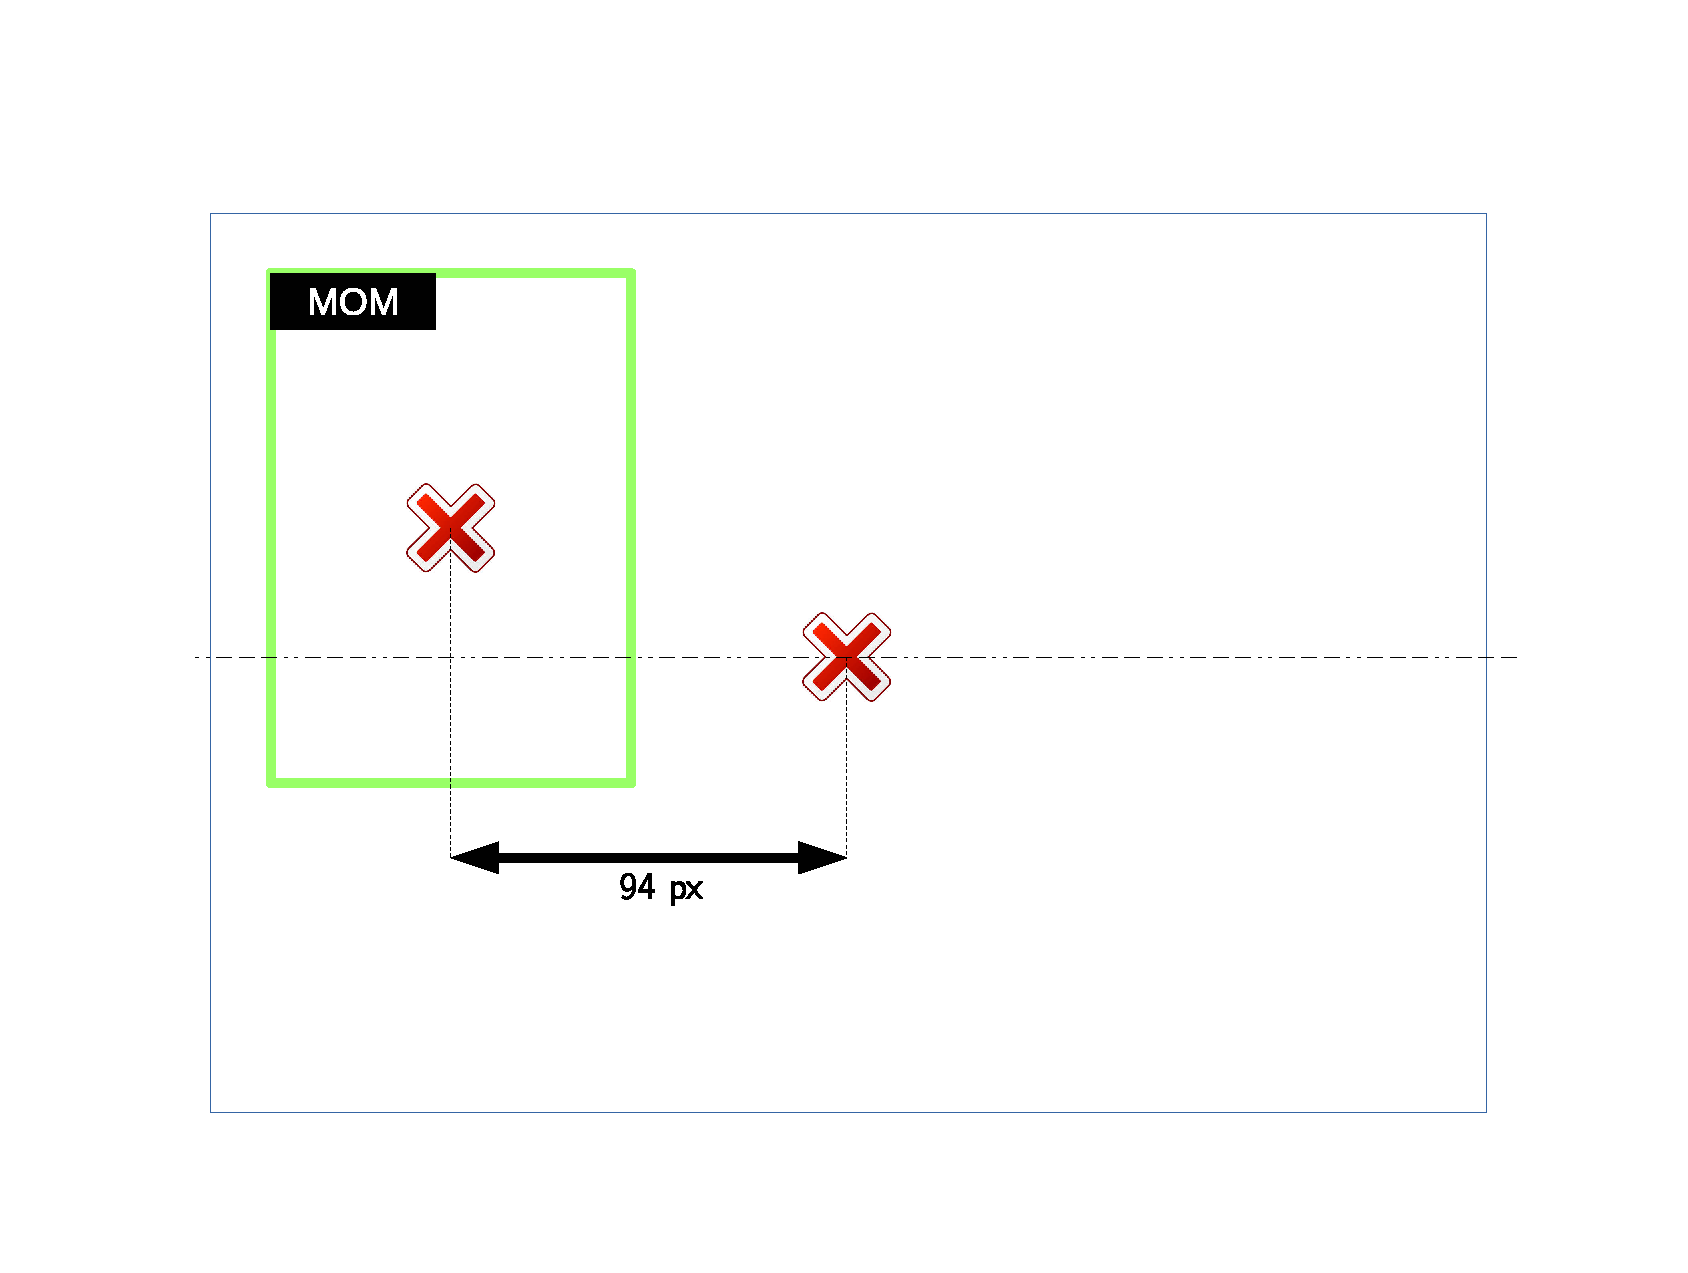
\includegraphics[width=3in]{images/h_error}
				\caption{Horizontal error estimation.}
				\label{fig:6_h_error}
			\end{subfigure}
			\hfill
			\begin{subfigure}[b]{0.5\linewidth}
				\centering
				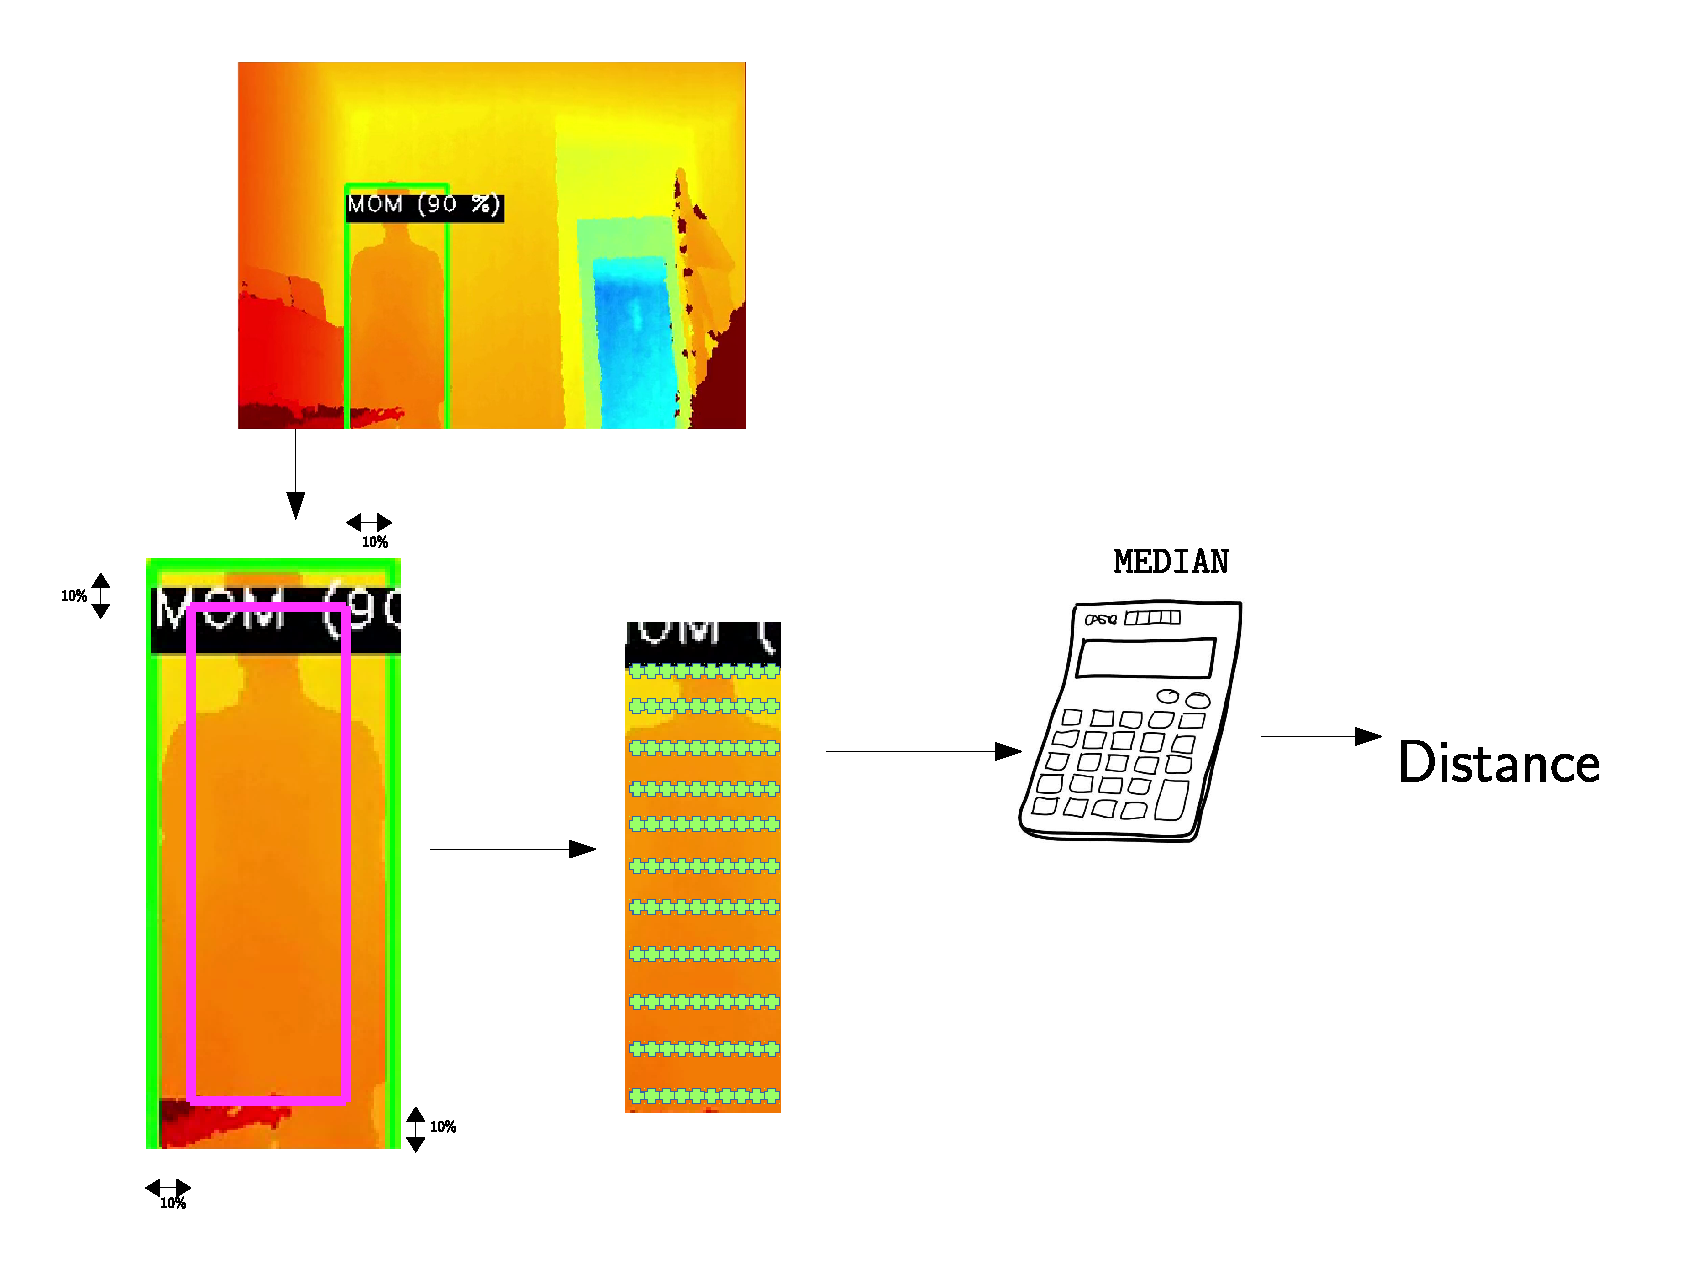
\includegraphics[width=3.7in]{images/distance_error}
				\caption{Computation of the median distance to \emph{mom}.}
				\label{fig:6_distance_to_mom}
			\end{subfigure}

			\caption{Computations of both errors.}
			\label{fig:6_errors}
		\end{figure}

	
	
	
	\subsection{PID controller}
		Once we know the relative \emph{mom}'s relative position from the robot, we have to send the proper commands to the robot, to make it follow \emph{mom}. On the first place, we have to know when to act and when to stop the motors. As we don't want the robot to go to the exact place where \emph{mom} is, we have to establish a \emph{safe/dead zones}, where we the robot won't move further towards \emph{mom}. These zones are represented in \autoref{fig:6_followperson_safe_zones}.\\
		
		\begin{figure}[h]
			\centering
			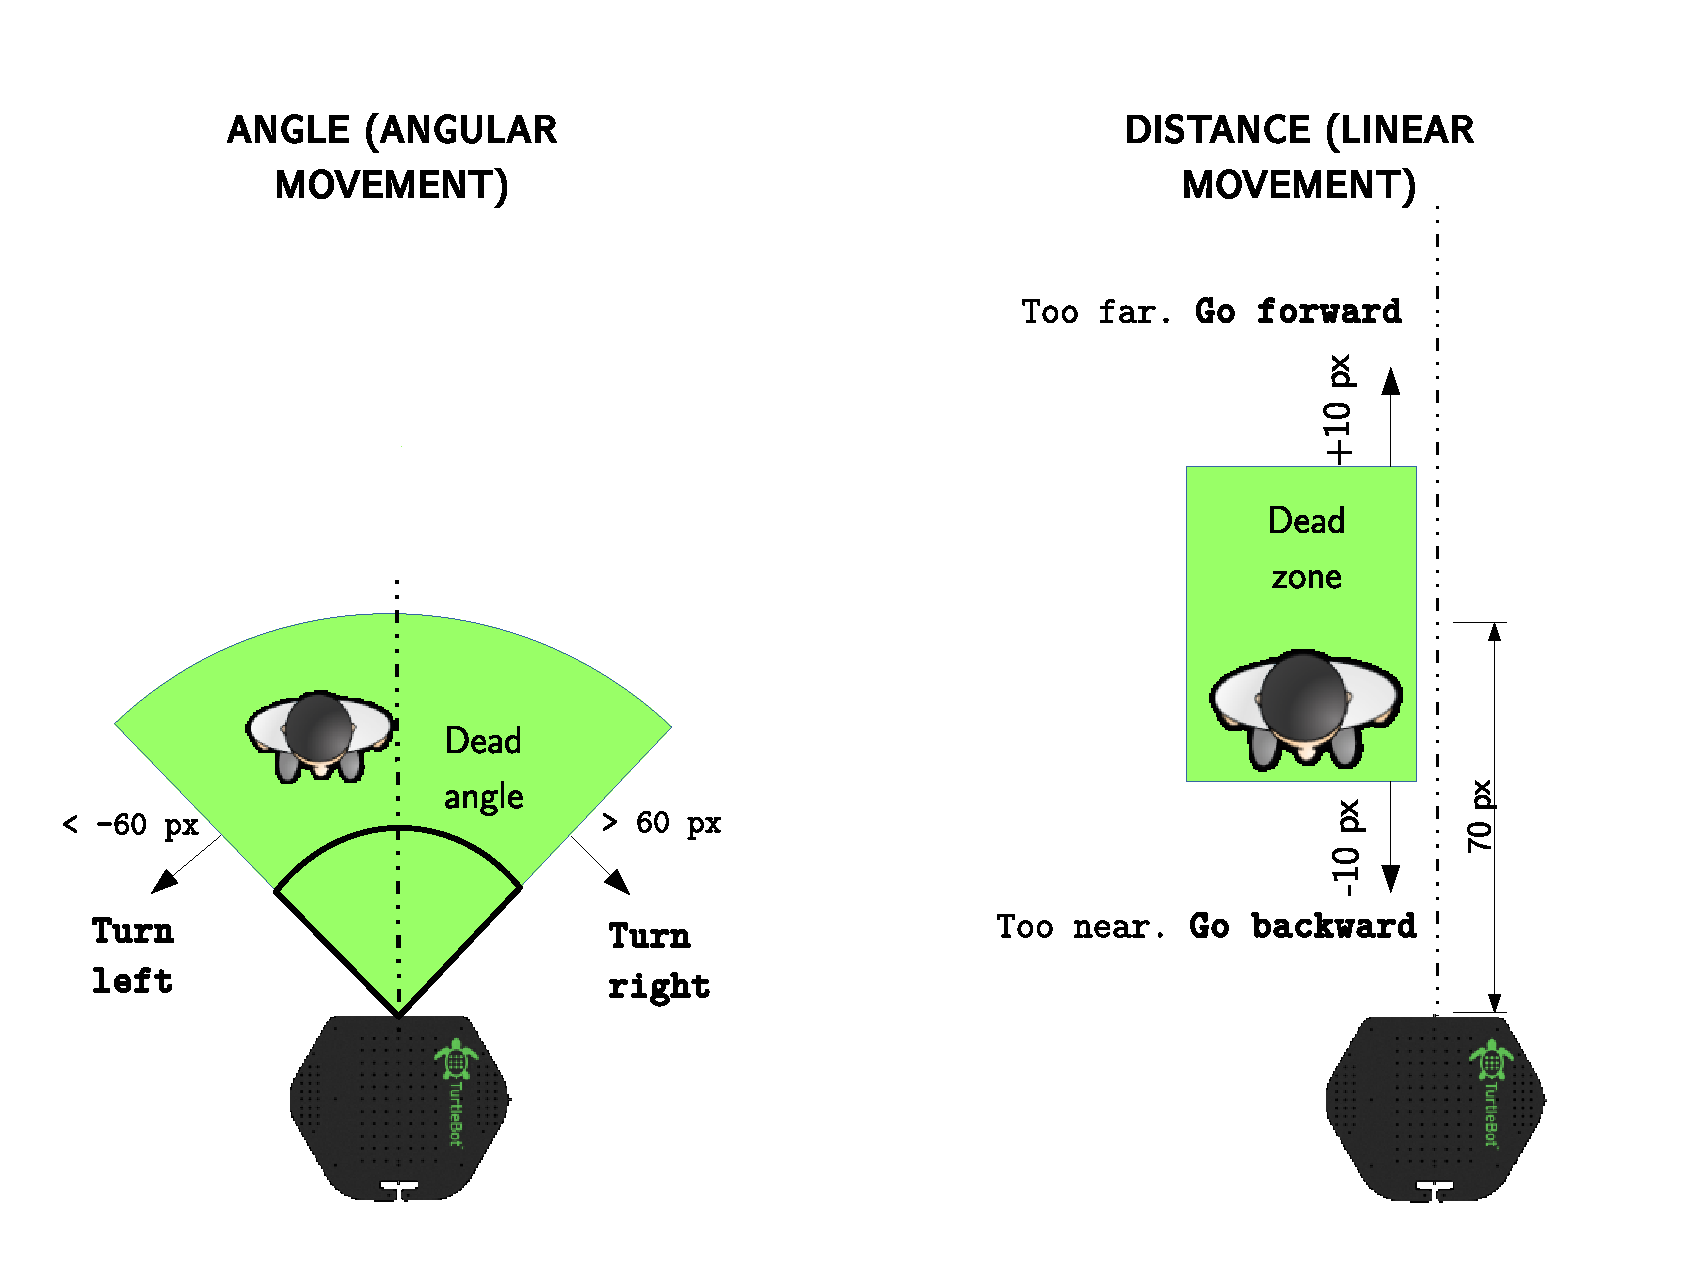
\includegraphics[width=4in]{images/followperson_movement_schema}
			\caption{Safe zones. The robot will consider \emph{mom} as correctly followed inside them (on a separate way for each dimension).}
			\label{fig:6_followperson_safe_zones}
		\end{figure}
	
			As our desirable relative position is to be aligned (the center of the bounding box in the center of the image) and at a safe distance (at $\pm$ 10 px from the reference distance), we will rotate and/or move in a straight line in consequence, trying to carry \emph{mom} inside the safe zones. Hence, we have to \emph{compute a proper response} to move the robot towards the correct direction (independent responses on the angular and linear dimensions). Instead of computing just a response on a proportional way to the current error, we can implement a \emph{closed loop feedback system}, which keeps in mind the previous readings and responses computed, to get a better fitting to the ideal response in that moment\footnote{Otherwise, we can suffer oscillations and peaks on the response, as this application is a system affected by noise and possible errors in the measure. That is the reason why we implemented all the past softening blocks.}. Concretely, we will implement a \emph{PID} controller \cite{pid:}, which is the most common form of feedback at industrial applications (more than 95\% of the control loops are of this kind). PID stands for \emph{Proportional, Integral and Derivative} control, and computes a total response ($u(t)$) following the next formula (modified for discrete time, as we are on a digital system):
			
			\begin{equation}
			u[n] = k_p e[n] \ \ + \ \ k_i \sum_{i=0}^{n}e[i] \ \ + \ \ k_d (e[n] - e[n-1])
			\label{eq:6_pid}
			\end{equation}
			
			For those who did not stop reading, we will analyze this formula, which combines three sub-responses:
			
			\begin{itemize}
				\item \emph{Proportional}: $k_p e[n]$. This is the basic component, that computes a response directly proportional to the measured error.
				
				\item \emph{Integral}: $k_i \sum_{i=0}^{n}e[i]$. Here we compute an additional response, equivalent to the summation of the total error until now. This way, although a proportional response is not enough and the error gets stabilized in a non-zero value, the system will accumulate that error, getting \emph{annoyed} with the time. So, we will get a bigger response the bigger the total error is\footnote{When the monitored variable goes into the tolerated zone again, the total error has to be reseted, as it won't be necessary for now.}.
				
				\item \emph{Derivative}: $k_d (e[n] - e[n-1])$. This part stands for the \emph{difference} between the last measured error and the current one, and it quantifies how is the system responding\footnote{On systems without inertia, this contribution is generally ignored, having a simple PI control loop instead.}. If the difference has a high value, that means that the system is on a far state/position with respect to the last iteration. So, in order to eliminate the \emph{inertia} the system could have acquired (which might bring oscillations and overshooting), the derivative part acts, braking or accelerating the command depending on the observed response to the previous one.
			\end{itemize}
			
			As we can see, the combination of the three responses can achieve a much faster and steadier response (\autoref{fig:6_pids}), bringing back the system under control on a fast and efficient way. Each contribution is parameterized by its corresponding constant ($k_c, k_i, k_d$), so a critical task is to find the optimum value for each one of them.\\
			
			For our implementation, as we have implemented two independent PID controllers (for linear and angular speeds, respectively), we have experimentally looked for the most suitable values for each one of the parameters, obtaining the combination on \autoref{tab:6_pids}. It is important to mention that these are not the final values that regulate the movement (as the angular and linear errors move in different scales, a difference of 1 pixel in the angular error means almost nothing, but much more in the linear one). For this reason, and to keep reasonable values, they are scaled by internal constants inside of each PID controller.
			
			\begin{table}[h]
				\centering
				\begin{tabular}{|c|c|c|}
					\hline
					\textbf{} & \textbf{Linear} & \textbf{Angular} \\ \hline
					$k_p$     & 2               & 7                \\ \hline
					$k_d$     & 0.1             & 0.5              \\ \hline
					$k_i$     & 3               & 10               \\ \hline
				\end{tabular}
				\caption{Optimal found values for the parameters in each PID controller.}
				\label{tab:6_pids}
			\end{table}
			
			As the rule that governs the controller is the same (\autoref{eq:6_pid}), we have created a generic class (\texttt{PIDDriver}), which controls a motor with a PID closed loop, adding extra functionalities as soft reactive responses (to avoid abrupt movements), and limiters in the response, to mantain control over the robot.\\
			
			
			
			
			 \begin{figure}[h]
			 	\centering
			 	\begin{subfigure}[b]{0.3\linewidth}
			 		\centering
			 		\includegraphics[width=2.2in]{images/pid_p}
			 		\caption{Proportional.}
			 		\label{fig:6_pid_p}
			 	\end{subfigure}
			 	\hfill
			 	\begin{subfigure}[b]{0.3\linewidth}
			 		\centering
			 		\includegraphics[width=2.2in]{images/pid_pi}
			 		\caption{PI.}
			 		\label{fig:6_pid_pi}
			 	\end{subfigure}
			 	\hfill
			 	\begin{subfigure}[b]{0.3\linewidth}
			 		\centering
			 		\includegraphics[width=2.2in]{images/pid_pid}
			 		\caption{Full PID.}
			 		\label{fig:6_pid_pid}
			 	\end{subfigure}
			 	\caption{Different controllers response along time.}
			 	\label{fig:6_pids}		 	
			 \end{figure}
		
	This way, we compute a suitable response with a PID controller for each dimension, and the mentioned class sends it directly to the motors (thank to the possibility of passing the move function as an argument to the generic controller).\\
	
	So finally, we have the final code schema of the functionality added in top of \emph{ObjectDetector}:
	
	
	\begin{lstlisting}
...
# jdrc is the comm communicator.

# We create the client to move the robot:
motors_publisher = jdrc.getMotorsClient('FollowPerson.Motors')
w_function = motors_publisher.motors.sendW
v_function = motors_publisher.motors.sendVX

# Controllers creation:
w_PID = PIDController(w_function,
                      Kp=_,
                      Ki=_,
                      Kd=_,
                      scaling_factor=_,
                      limiter=_)

w_PID = PIDController(w_function,
                      Kp=_,
                      Ki=_,
                      Kd=_,
                      scaling_factor=_,
                      limiter=_)
...

# Measure of the errors:
angular_error = [subtract centers]
linear_error = [sample depth of person]

# Computation of the response (PID controllers):
w = w_PID.computeResponse(angular_error)
v = v_PID.computeResponse(linear_error)

# The controllers automatically send the response on a
# reactive but soft way.
	\end{lstlisting}

	At the end of the each iteration, we get the robot moved towards \emph{mom} (the target person to follow), making use of all the previously defined blocks (\autoref{fig:6_followperson_final}), as it can be seen on the final result, posted on the project Wiki\footnote{\url{http://jderobot.org/Naxvm-tfg}}.


	\begin{figure}[h]
		\centering
		\includegraphics[width=5in]{images/followperson_general_schema}
		\caption{Functional diagram of the \texttt{FollowPerson} node.}
		\label{fig:6_followperson_final}
	\end{figure}

\section{Experiment: PTZ Camera}
	\label{sec:follow_ptz}
	As an alternative experiment or approach, we can implement this tracking and following system on a PTZ camera. As explained in \autoref{sec:3_ptz}, these cameras are supported by servo motors on vertical and horizontal axis, that allow the camera to move as a \emph{mechanical neck}.\\
	
	We can consider an alternative system, which implements the previous pipeline (with slight modifications), using this camera (Sony EVI D100P, on \autoref{fig:3_evi}) as the \emph{actuator device}. Thank to the Python distribution easiness using packages, this case can be implemented as an additional package, being able to modify as less as possible. So, \texttt{FollowPerson} commutes pertinent functions between the Turtlebot and the PTZ packages in runtime, just selecting the used device in the YML file.\\
	
	The movement commands are now destinated to pure \emph{rotations} of the neck, so the movement update on each axis (vertical/horizontal) has to be computed on a similar way than the horizontal case on the Turtlebot (\autoref{fig:6_h_error}). So, our approach in this case follows the computation on \autoref{fig:6_ptz_error}
	
	
	\begin{figure}[h]
		\centering
		\begin{subfigure}[b]{0.6\linewidth}
			\centering
			\includegraphics[width=4in]{images/ptz_error_comp}
			\caption{Error computation on each axis.}
			\label{fig:6_ptz_error}
		\end{subfigure}
		\hfill
		\begin{subfigure}[b]{0.5\linewidth}
			\centering
			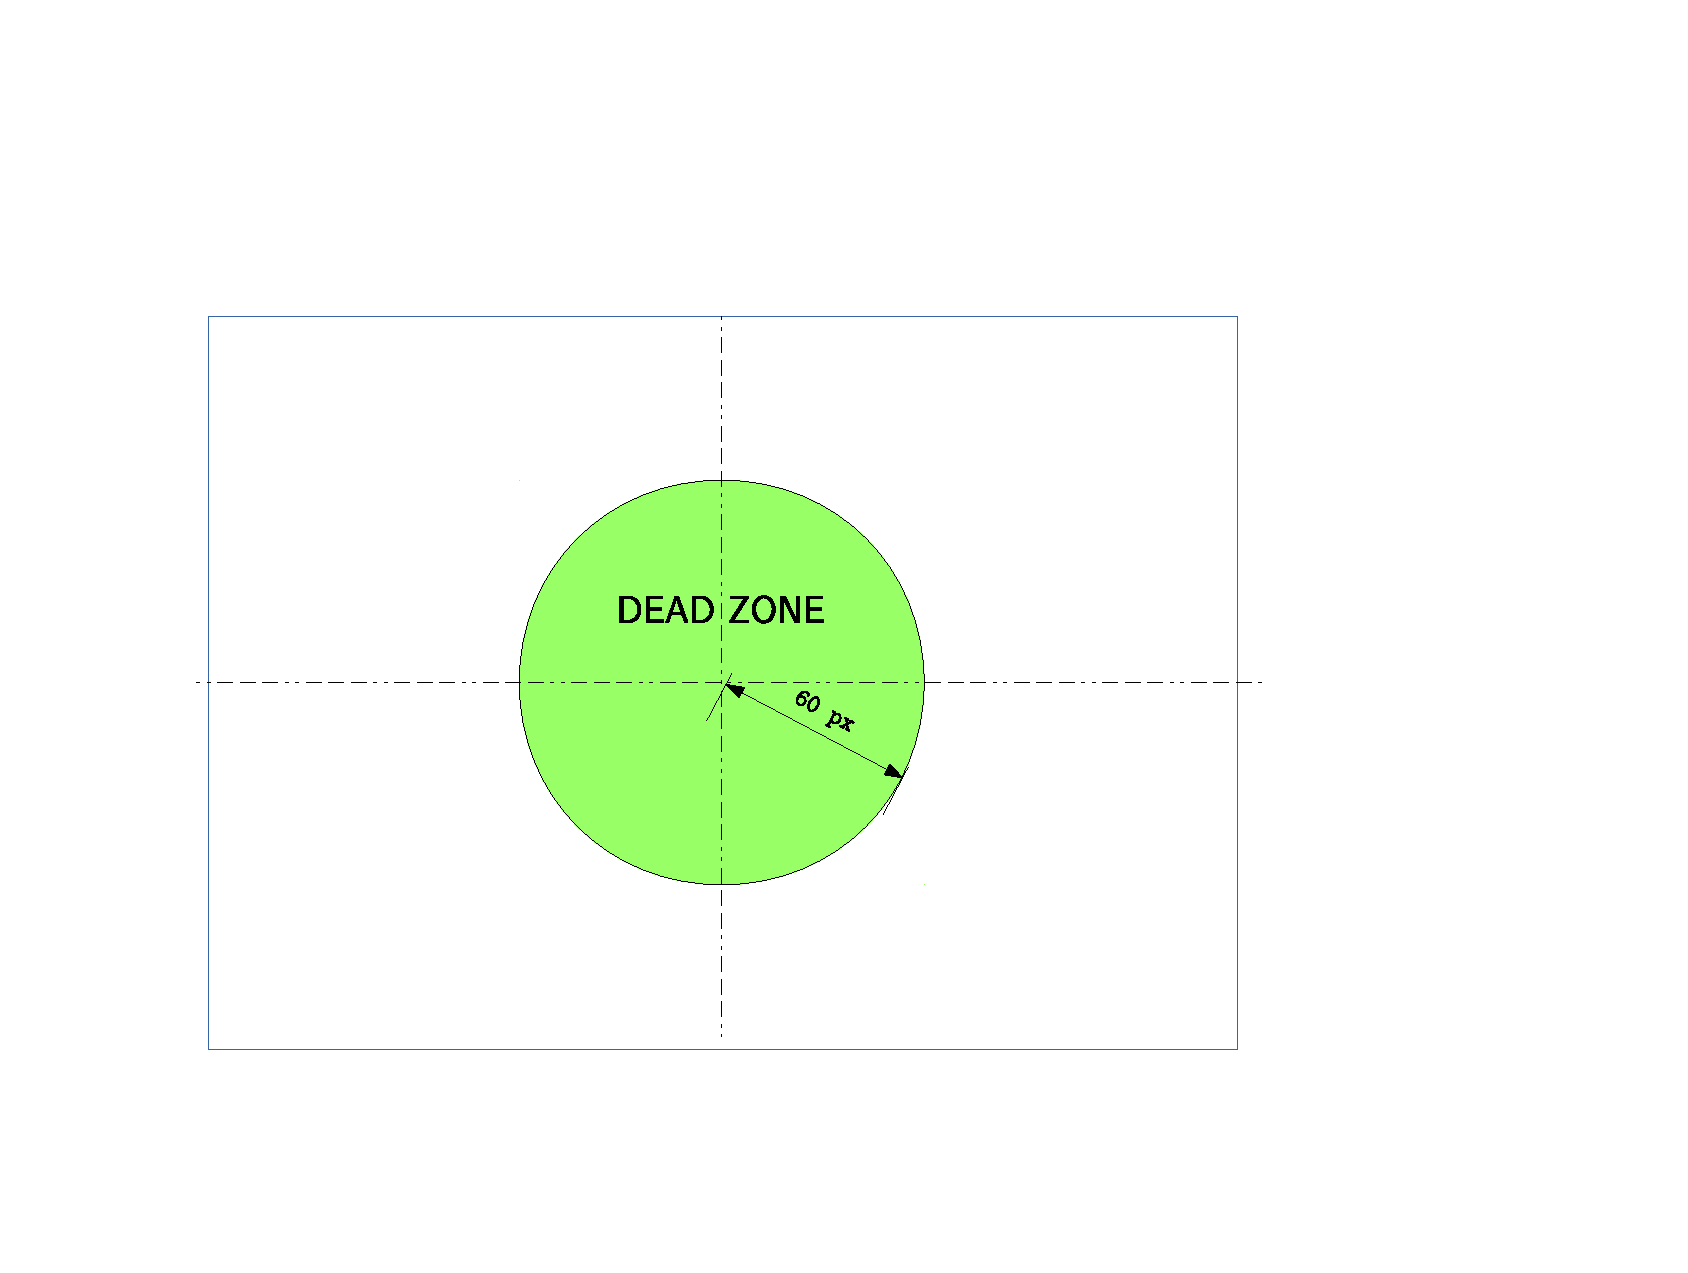
\includegraphics[width=4in]{images/ptz_dead_zone}
			\caption{Dead zone of actuation (radius of 60 px).}
			\label{fig:6_ptz_dead_zone}
		\end{subfigure}
		\caption{Error computation parameters on the PTZ case.}
		\label{fig:6_ptz_parameters}
	\end{figure}
	
	However, as the movement commands are stored in a queue buffer, we are limited to perform \emph{differential} pose updates (e.g. move 1 or 2 degrees on each axis towards the objective per iteration), as described in \autoref{fig:3_ptz_movements}. Hence, a PID controller does not make sense here, as the set of feasible outputs is discrete and non adjustable:
	\begin{itemize}
		\item $0$ if the error stays inside the dead zone (\autoref{fig:6_ptz_dead_zone}).
		
		\item $\pm 1$ if the system lost \emph{mom} (in order to slowly move looking for it).
		
		\item $\pm 2$ if mom is being tracked. The camera performs an increment of that magnitude towards mom in each axis.
	\end{itemize}
	

	Finally, we can take advantage of the most of the standard \texttt{FollowPerson} total algorithm, obtaining the schematic algorithm on \autoref{fig:6_ptz_total}.
	
	
	\begin{figure}[h]
		\centering
		\includegraphics[width=5.5in]{images/ptz_general_schema}
		\caption{Total schema followed in the PTZ case.}
		\label{fig:6_ptz_total}
	\end{figure}